\section{Related Works}
In this section, we summarize two lines of literature that are most relevant to ours.

\subsection{CoT Prompting}
The recent surge in computational power has paved the way for the rise of expansive language models. With increasing complexity, these models have unlocked emerging capabilities, notably in-context learning and CoT reasoning \cite{wei2022chain,brown2020language,schaeffer2023emergent}.

In their seminal work, Brown et al. discovered the ability of large-scale language models to leverage in-context learning (ICL)~\cite{brown2020language}. ICL strategy involves weaving input-output examples directly into the prompt, allowing ready-to-use large language models to perform impressively without the need for task-specific fine-tuning. However, despite its promise, this end-to-end methodology often falters when confronting complex reasoning challenges.

Building on this, \citeauthor{wei2022chain} demonstrated that integrating a series of logical reasoning steps into the model demonstrations, called CoT prompting, significantly refines the reasoning capabilities of large language models \cite{wei2022chain}. CoT prompting not only deepens the model's grasp of the nuanced questions and their underlying logic but also yields an articulated sequence of reasoning steps. Zhang et al.'s ``Auto-CoT" method represents a significant advancement in the field of AI reasoning \cite{zhang2022automatic}. By automating the CoT process, it addresses complex problems more effectively.
%
And then Yao et al. introduced the ``Tree of Thoughts" (ToT) framework, an evolution of the Chain of Thought approach for language model inference \cite{yao2023tree}. ToT allows language models to explore different units of text as intermediate steps in problem-solving. This framework enables more deliberate decision-making by considering multiple reasoning paths.
%
\subsection{Preliminary Work on Analyzing CoT}
The development and understanding of CoT reasoning in AI have evolved over time, marked by significant contributions from various researchers. Initially, Madaan and Yazdanbakhsh \cite{madaan2022text} explored the decomposition of prompts into symbols, patterns, and texts, examining the effects of CoT through counterfactual prompting. This study laid the groundwork for understanding how different components of a prompt influence AI reasoning.
Besides, several studies furthered this understanding. Tang et al. \cite{tang2023large} investigated the role of semantics in CoT reasoning, uncovering a reliance on semantic knowledge from pre-training and challenges in symbolic reasoning. Around the same time, Wang et al. focused on the impact of demonstration selection in CoT, revealing that the relevance and order of reasoning are more critical than the accuracy of reasoning chains \cite{wang2023selfconsistency}.

Theoretical perspectives also emerged recently, offering deeper insights into the mechanics of CoT. For example, Li et al. conceptualized CoT as a multi-step combinatorial function, illustrating its role in simplifying in-context learning for complex questions~\cite{li2023dissecting}. Feng et al. theoretically demonstrated the sufficiency of a fixed-size Transformer for computational tasks and dynamic planning within CoT frameworks~\cite{fu2023complexitybased}.

Further contributions in this field included those of Merrill and Sabharwal, who observed that CoT can improve reasoning abilities, with improvements scaling with the number of intermediate steps \cite{merrill2023expressive}. Wu et al. employed gradient-based feature attribution methods to assess the robustness of CoT against question variations and perturbations \cite{wu2023analyzing}.

\begin{figure*}[ht]
    \centering
    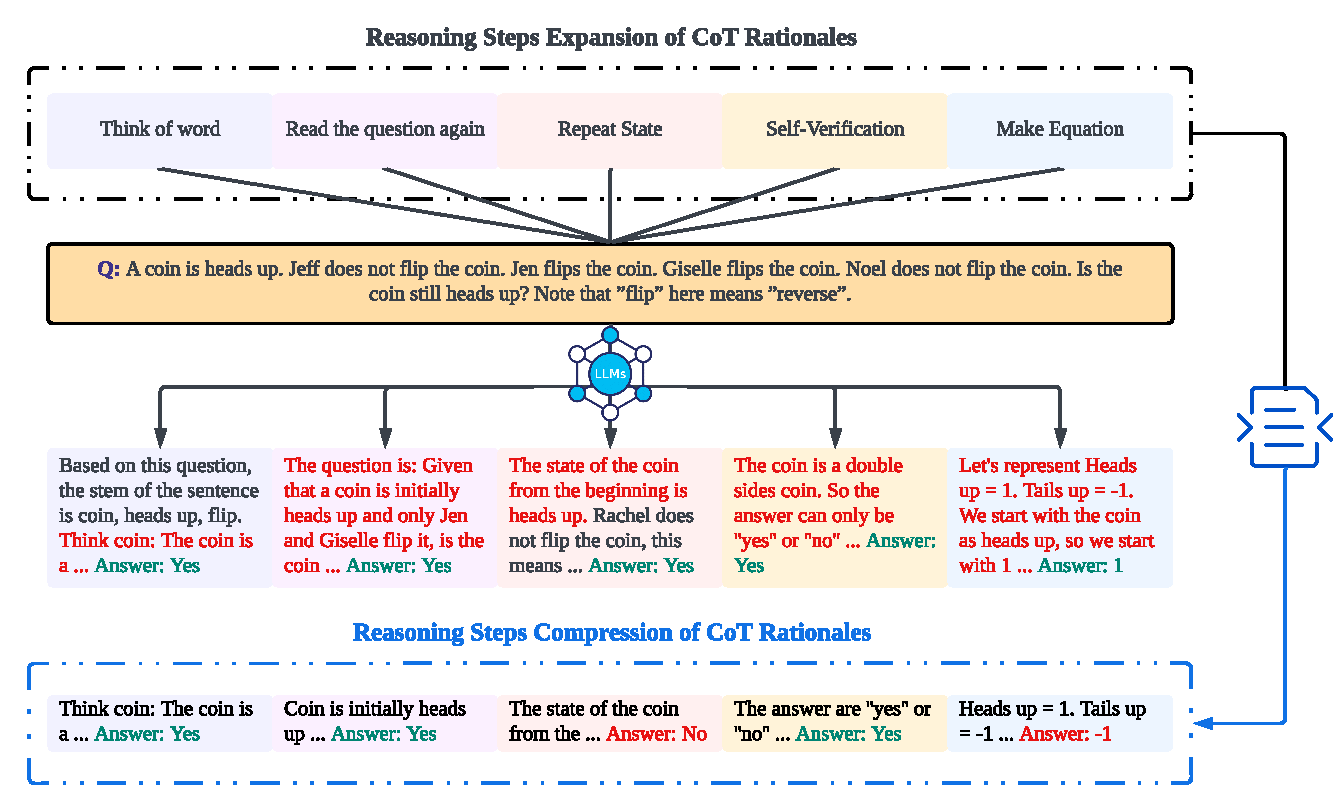
\includegraphics[width=1\linewidth]{intro.pdf}
    \caption{Increase the length of the thinking chain through the method in the figure, and compress the thinking chain without losing information as much as possible.}
    \label{fig:intro}
\end{figure*}